%%%%%%%%%%%%%%%%%%%%%%%%%%%%%%%%%%%%%%%%%
% Beamer Presentation
% LaTeX Template
% Version 1.0 (10/11/12)
%
% This template has been downloaded from:
% http://www.LaTeXTemplates.com
%
% License:
% CC BY-NC-SA 3.0 (http://creativecommons.org/licenses/by-nc-sa/3.0/)
%
%%%%%%%%%%%%%%%%%%%%%%%%%%%%%%%%%%%%%%%%%

%----------------------------------------------------------------------------------------
%	PACKAGES AND THEMES
%----------------------------------------------------------------------------------------

\documentclass{beamer}

\mode<presentation> {

% The Beamer class comes with a number of default slide themes
% which change the colors and layouts of slides. Below this is a list
% of all the themes, uncomment each in turn to see what they look like.

%\usetheme{default}
%\usetheme{AnnArbor}
%\usetheme{Antibes}
%\usetheme{Bergen}
%\usetheme{Berkeley}
%\usetheme{Berlin}
%\usetheme{Boadilla}
%\usetheme{CambridgeUS}
%\usetheme{Copenhagen}
%\usetheme{Darmstadt}
%\usetheme{Dresden}
%\usetheme{Frankfurt}
%\usetheme{Goettingen}
%\usetheme{Hannover}
%\usetheme{Ilmenau}
%\usetheme{JuanLesPins}
%\usetheme{Luebeck}
\usetheme{Madrid}
%\usetheme{Malmoe}
%\usetheme{Marburg}
%\usetheme{Montpellier}
%\usetheme{PaloAlto}
%\usetheme{Pittsburgh}
%\usetheme{Rochester}
%\usetheme{Singapore}
%\usetheme{Szeged}
%\usetheme{Warsaw}

% As well as themes, the Beamer class has a number of color themes
% for any slide theme. Uncomment each of these in turn to see how it
% changes the colors of your current slide theme.

%\usecolortheme{albatross}
%\usecolortheme{beaver}
%\usecolortheme{beetle}
%\usecolortheme{crane}
%\usecolortheme{dolphin}
%\usecolortheme{dove}
%\usecolortheme{fly}
%\usecolortheme{lily}
%\usecolortheme{orchid}
%\usecolortheme{rose}
%\usecolortheme{seagull}
%\usecolortheme{seahorse}
%\usecolortheme{whale}
%\usecolortheme{wolverine}

%\setbeamertemplate{footline} % To remove the footer line in all slides uncomment this line
%\setbeamertemplate{footline}[page number] % To replace the footer line in all slides with a simple slide count uncomment this line

%\setbeamertemplate{navigation symbols}{} % To remove the navigation symbols from the bottom of all slides uncomment this line
}

\usepackage{graphicx} % Allows including images


\begin{document}

% Objective
\begin{frame}{Objective}
\textbf{\emph{Develop a machine-learning algorithm that uses mobile phone data to estimate gendered 
patterns and gaps in key labor market indicators in Ghana.}}
\end{frame}

% Labor Market Indicators
\begin{frame}{Labor Market Indicators}
\footnotesize
\begin{center}
\begin{tabular}{p{3.2cm} p{3.5cm} p{2.5cm}} 
\hline
Domain & Example Outcome & Outcome Type \\ \hline
Work & Hours worked in last 7 days & Continuous \\ 
Labor under-utilization & Under-employed in last 7 days & Binary \\ 
Informal Work & Worked informally in last 7 days & Binary \\ 
Commuting & Minutes spent during typical morning commute & Continuous \\ \hline
\end{tabular}
\end{center}
\end{frame}

% Joint Prediction
\begin{frame}{Joint Prediction}
\begin{itemize}
\item For each indicator, we want to estimate the expected value of the indicator for men and 
women, or $E(y \mid \delta = 0)$ and $E(y \mid \delta = 1)$.
\item Gender is unobserved, so we must jointly predict $y_i$ and $\delta_i$ for each person $i$.
\item The previously-used procedure is as follows:
\begin{enumerate}
\item With the training data, estimate a model that predicts gender.
\item With the training data, estimate two models that predict the indicator of interest, one model 
for each gender.
\item Apply the model from (1) to the test data and apply the models in (2) depending on the 
predicted value from (1).
\item Calculate gender-disaggregated labor market indicators.
\end{enumerate}
\end{itemize}
\end{frame}

% Limitations
\begin{frame}{Limitations}
\begin{enumerate}
\item Theoretical justification
% What is the rationale for the procedure? Why should we expect it to give good estimates?
\item Sample splitting
% The second stage splits the sample roughly in half, meaning each model is estimated with
% limited information
\item Error propagation
% Any prediction errors from the first stage will get passed onto the second stage
\item Correlated outcomes
% The single-output approach neglect correlation between the outcomes (e.g., the first stage
% completely ignores labor market indicators when estimating gender).
\item Uncertainty intervals
% The existing approach doesn't tell us anything about the uncertainty of the estimates.
\end{enumerate}
\end{frame}


\begin{frame}{Single-Output Prediction Model}{Bayesian additive regression tree (BART)}
\begin{itemize}
\item Univariate, nonparametric prediction tool
\item Sum of T 'weak learner' trees % that leads to robust out-of-sample predictions
\item Dynamically learns important predictors via a sparsity inducing prior
%\item Excels when $x$ is high in dimension, with relatively few important predictors


Mathematically, a BART model looks like:

\begin{align*}
Y_i &\sim N(\mu_i, \sigma^2)\\
\mu_i &= \sum_{t=1}^T g(x_i ; \tau_t, M_t)%\sum_{l \in L_t}\psi_{lt}I(x_i \leadsto (t,l))
\end{align*}


\item $g()$ tree function which inputs $x$ and outputs prediction
\item $\tau_t$: the $t^{th}$ tree structure in the forest 
\item $M_t$: node parameters for $t^{th}$ tree
\end{itemize}

%$I(x_i \leadsto (t,l)) = 1$ if $x_i$ falls into node ($t,l$) of tree $t$; 0 otherwise. 

\end{frame}

\begin{frame}{Multi-Output Prediction Model}{Shared Forest}
\begin{itemize}
\item An extension of BART for multivariate responses
\item Correlation between responses is utilized via shared tree structures
\item Assumption: variables that predict $Y_1$ are the same variables that predict $Y_2$ (though the nature of the relationship may be different!)
\item Information sharing $\Rightarrow$ better predictions for $Y_1$ \textit{and} $Y_2$ 
\item Can model binary and/or continuous outcomes
\end{itemize}
\end{frame}



\begin{frame}{Multi-Output Prediction Model}{1 binary, 1 continuous }

The shared forest package accomodates heterogeneous outcomes. 
\begin{itemize}
\item[ex)] $Y = $ hours worked, $\delta = $ gender
\end{itemize}
\begin{align*}
Y_i &\sim N(\mu_i, \sigma^2_i) \\
\delta_i &\sim Bernoulli(\pi_i)
\end{align*}

\begin{itemize}
\item $\begin{pmatrix}\mu_i & \pi_i \end{pmatrix}$ modeled jointly using a shared forest model

$$\begin{pmatrix}\mu_i \\ \Phi^{-1}(\pi_i) \end{pmatrix} = 
\begin{pmatrix}\sum_{t=1}^T g(x_i ; \tau_t, M^{\mu}_t)\\%\sum_{l \in L_t}\psi_{lt}I(x_i \leadsto (t,l)) \\ 
\sum_{t=1}^T g(x_i ; \tau_t, M^{\theta}_t)%\sum_{l \in L_t}\theta_{lt}I(x_i \leadsto (t,l))
\end{pmatrix} $$

where $\Phi^{-1}$ is the probit link function.
\end{itemize}
\end{frame}


\begin{frame}{Multi-Output Prediction Model}{1 binary, 1 continuous }
\begin{itemize}
\item ``Information sharing": likelihood for $\tau_t$ involves two dimensional response: $\{Y_i, \delta_i\}_{i = 1}^N$
\item Algorithm's decisions about tree structure ($\tau_t$) considers what is beneficial to both $Y$ and $\delta$
\item Predictions of $\delta$ are improved by utilizing information provided by $Y$, vice versa
\end{itemize}
\end{frame}


\begin{frame}{Multi-Output Prediction Model}{2 binary responses}
%The model structure is the same as described before; however, the likelihood reflects that:

In our application, we may have two binary responses
\begin{itemize}
\item[ex)] $\delta_1$ = gender, $\delta_2$ = employed
\end{itemize}


\begin{align}
\delta_{1i} &\sim Bernoulli(\pi_{1i}) \\
\delta_{2i} &\sim Bernoulli(\pi_{2i})
\end{align}

As before, the tree structures will be built using information shared between $\delta_1$ and $\delta_2$, while the location parameters are estimated separately. 

$$\begin{pmatrix}\Phi^{-1}(\pi_{1i}) \\ \Phi^{-1}(\pi_{2i}) \end{pmatrix} = 
\begin{pmatrix}\sum_{t=1}^T g(x_i ; \tau_t, M^{1}_t)\\%\sum_{l \in L_t}\psi_{lt}I(x_i \leadsto (t,l)) \\ 
\sum_{t=1}^T g(x_i ; \tau_t, M^{2}_t)%\sum_{l \in L_t}\theta_{lt}I(x_i \leadsto (t,l))
\end{pmatrix} $$


\end{frame}


\begin{frame}{Simulation Study }{1 binary, 1 continuous}
We run 100 simulations. In each:
\begin{itemize}
\item $n_{train} = 500$, $n_{test} = 500$
%\item We set the number of covariates to P = 150. 
\item Predictors: $x_1, \hdots, x_{150} \sim Unif(0,1)$
\item True underlying means based on a modification of the ``Friedman function"
\begin{align*}
y_i &= 10 \sin (\pi x_{1i} x_{2i}) + 20(x_{3i} - 0.5)^2 + 10x_{4i} + 5x_{5i} +
\epsilon_i^Y\\
\delta_i &= \begin{cases}1 &\text{ if }5 \sin (\pi x_{1i} x_{2i}) + 25(x_{3i} - 0.5)^2 + 5x_{4i} + 10x_{5i} +
\epsilon_i^{\delta} > 0 \\
                          0 & \text{ otherwise}\end{cases}
\end{align*}

where $(\epsilon_i^Y, \epsilon_i^{\delta}) \overset{iid}{\sim} N(0,1)$

\end{itemize}



\end{frame}

\begin{frame}{Simulation Study}{1 binary, 1 continuous }
Two quantities may be of interest for prediction
\begin{enumerate}
\item $E( y_i^* \mid x_i)$,$E(\delta_i^* \mid x_i)$, where $^*$ indicates those observations come from a test / hold-out sample
  \begin{itemize}
    \item[ex)] Predict hours worked for individual, conditional on cellular traits $x_i$
    \item[ex)] Predict gender of individual, conditional on cellular traits $x_i$
  \end{itemize}
\item $E(y^* \mid \delta = 1) = \frac{1}{\sum I(\delta_i = 1)}\sum_{i: \delta_i = 1}E(y_i^* \mid x_i)$
  \begin{itemize}
    \item[ex)] Predict mean hours worked for females (avg. across traits observed for females, i.e., $\delta = 1$)
    \item[ex)] Predict mean hours worked for males (avg. across traits observed for males, i.e., $\delta = 0$)
  \end{itemize}
\end{enumerate}
\end{frame}


\begin{frame}{Predicting Individual $Y^*$ }{One typical simulation}
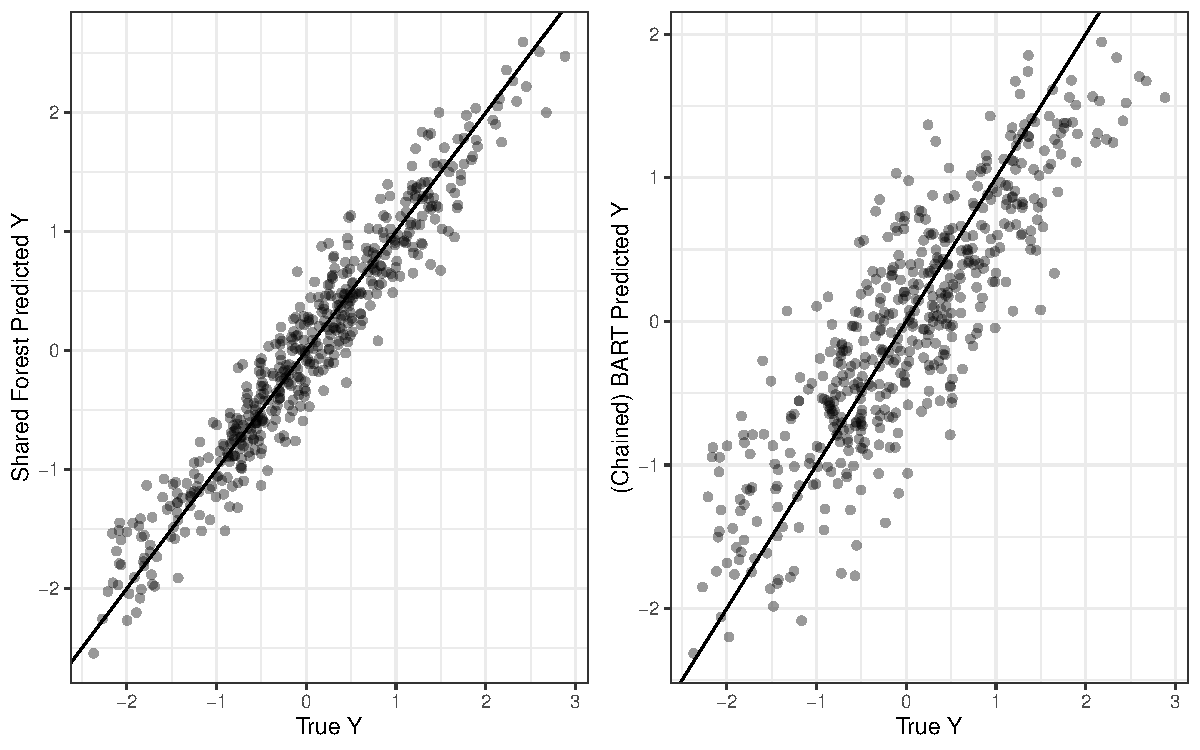
\includegraphics[width = .9\linewidth]{continuous_sim_results_single_sim.pdf}
\end{frame}

\begin{frame}{Predicting Individual $Y^*$ }
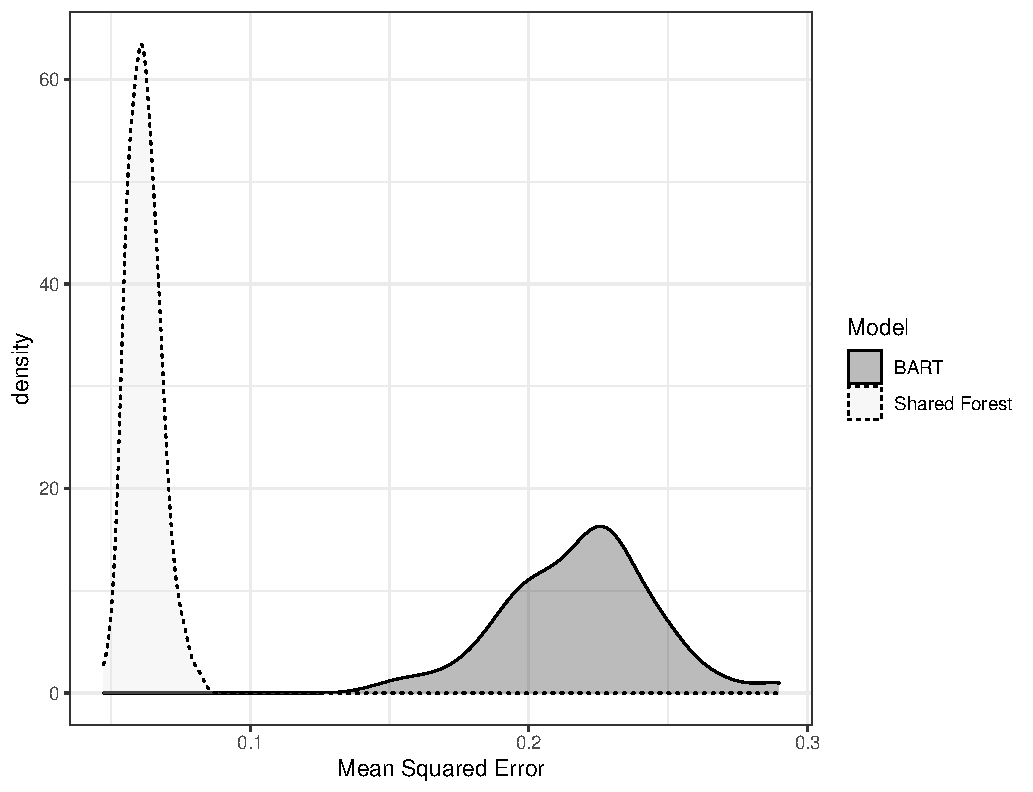
\includegraphics[width = .9\linewidth]{continuous_sim_results_ind_y.pdf}
\end{frame}


\begin{frame}{Predicting Individual $\delta*$}
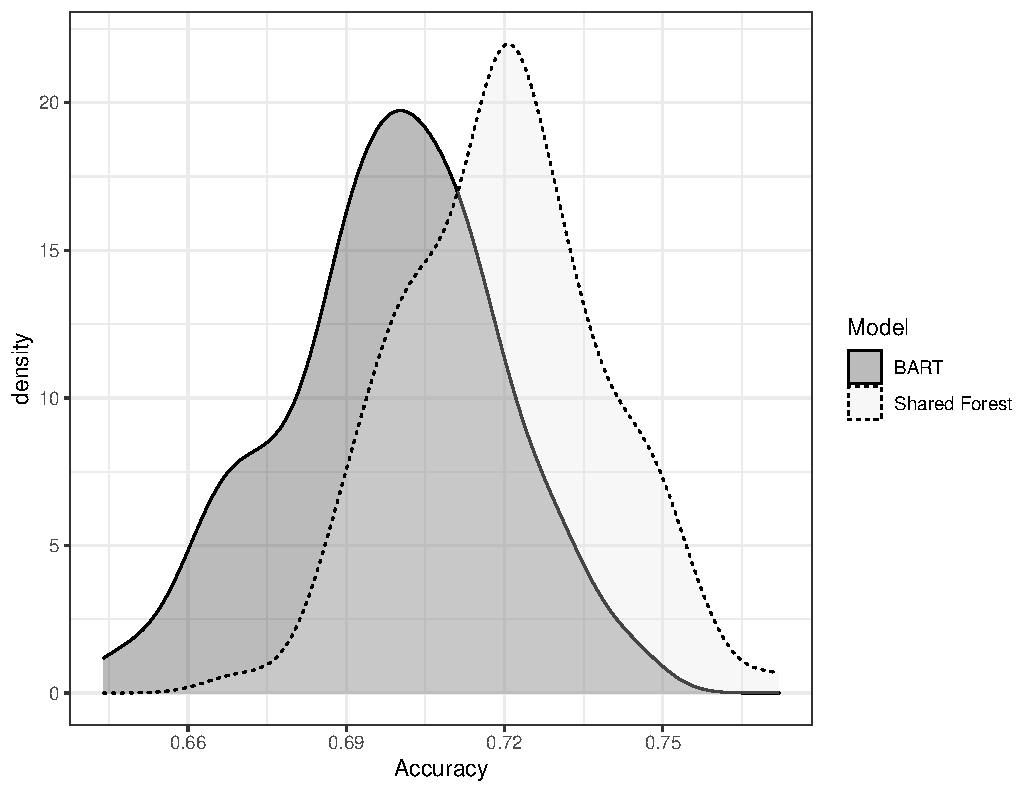
\includegraphics[width = .9\linewidth]{continuous_sim_results_ind_delta.pdf}
\end{frame}


\begin{frame}{Predicting $E(Y^* \mid \delta^*)$ }
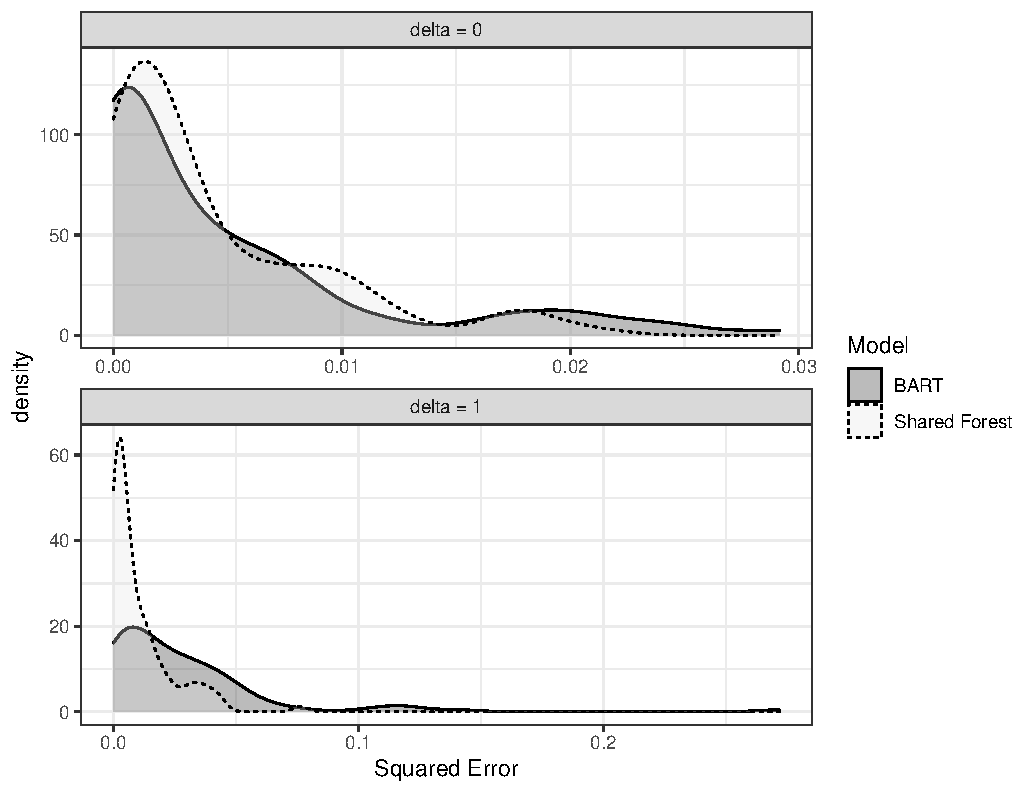
\includegraphics[width = .9\linewidth]{continuous_sim_results.pdf}
\end{frame}

\begin{frame}{Predicting $E(Y^* \mid \delta^*)$ }

% latex table generated in R 4.0.5 by xtable 1.8-4 package
% Tue Mar  1 10:17:05 2022
\begin{table}[ht]
\centering
\begin{tabular}{rlr}
  \hline
$\delta$ & Model & MSE\\
  \hline
0 & BART & 0.004875  \\ 
  0 & Shared Forest & 0.004330  \\ 
  1 & BART & 0.028464  \\ 
  1 & Shared Forest & 0.010399  \\ 
   \hline
\end{tabular}
\caption{\label{tab:mse} Mean of the squared errors (across simulations) comparing the true $E(Y^* \mid \delta^*)$ to the estimated $\hat{E}(Y^* \mid \hat{\delta})$.}
\end{table}

\end{frame}




\begin{frame}{2 binary responses}
\begin{itemize}
\item In this context, we are interested in predicting $P(\delta^*_2=1 \mid \delta^*_1)$.
\begin{itemize}
\item[ex)] Probability a randomly selected female is employed. \\($\delta_1$ = gender, $\delta_2$ = employment)
\end{itemize}
\item We measure model performance by looking at the squared errors comparing the true population (conditional) means to the estimated. 

\item The simulation study is identical, but with two binary responses. Importantly, these responses again have differing mean functions. 
\end{itemize}
\end{frame}

\begin{frame}{Predicting $E(\delta_2^* \mid \delta_1^*)$ }
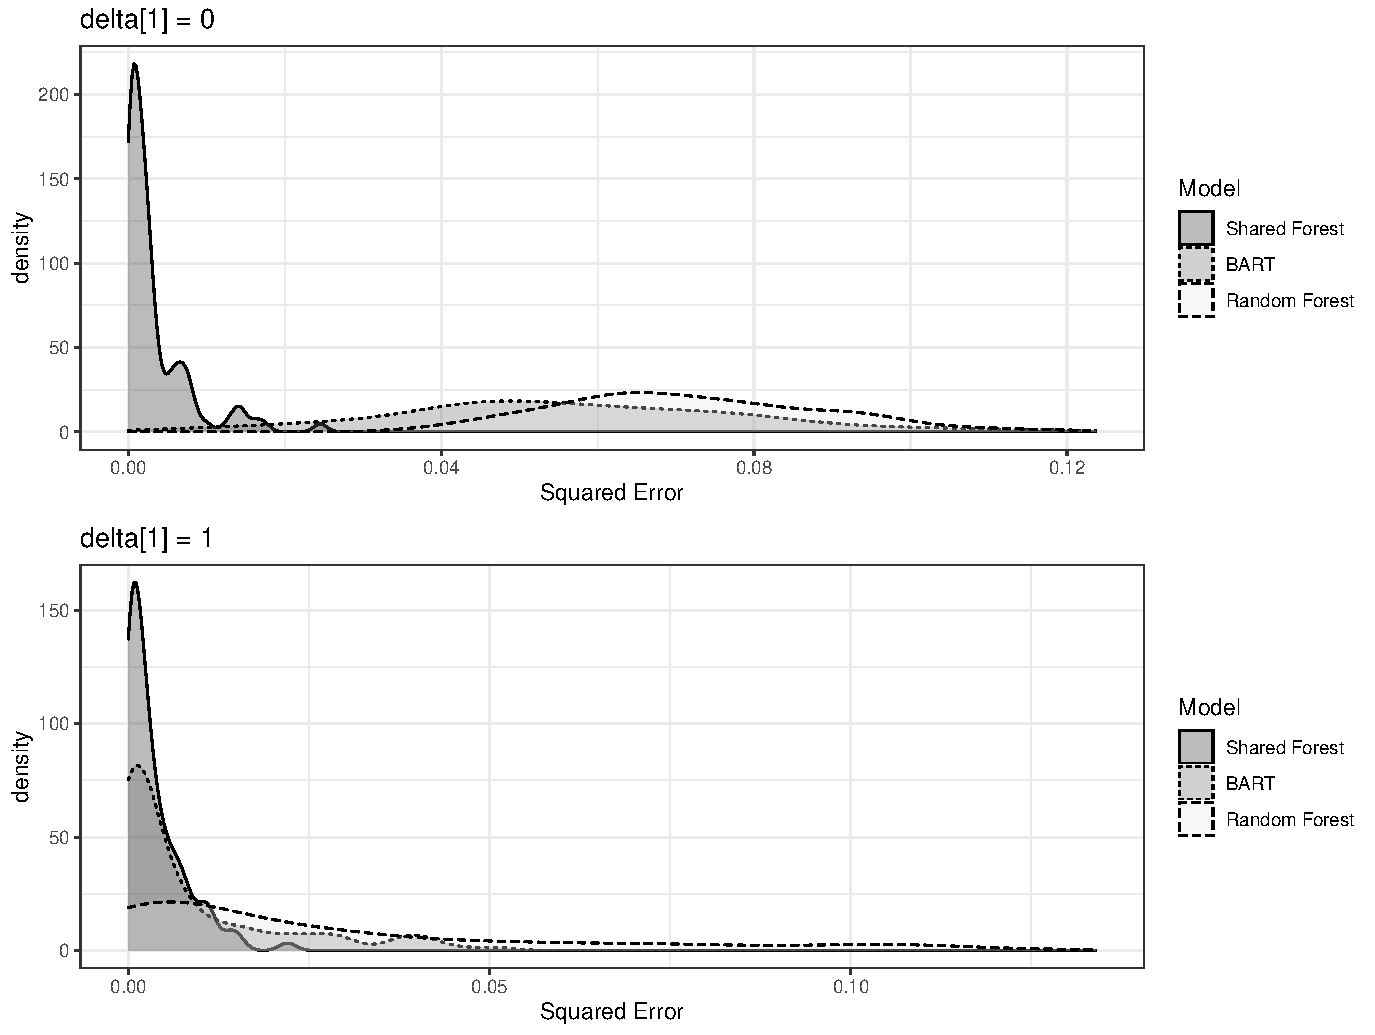
\includegraphics[width = .9\linewidth]{binary_sim_results.pdf}
\end{frame}

\begin{frame}{Predicting $E(\delta_2^* \mid \delta_1^*)$ }
% latex table generated in R 4.0.5 by xtable 1.8-4 package
% Fri Mar  4 08:55:46 2022
\begin{table}[ht]
\centering
\begin{tabular}{lrr}
  \hline
Model & MSE & $\delta_1$ \\ 
  \hline
BART & 0.056580 & 0 \\ 
  Random Forest & 0.071952 & 0 \\ 
  Shared Forest & 0.003252 & 0 \\ \hline
  BART & 0.008327 & 1 \\ 
  Random Forest & 0.027744 & 1 \\ 
  Shared Forest & 0.003514 & 1 \\ 
   \hline
\end{tabular}
\end{table}
\end{frame}


\end{document}